\documentclass[11pt]{article}
\usepackage[margin=1in]{geometry}
\usepackage{amsmath,amssymb,amsthm,bm}
\usepackage{hyperref}
\usepackage{graphicx}
\usepackage{caption}
\usepackage{listings}
\usepackage{xcolor}
\usepackage{float}
\usepackage{placeins}

% Graphics path
\graphicspath{{figures/}}

% Listings style for code
\lstdefinestyle{code}{%
  language=Python,
  basicstyle=\ttfamily\small,
  numbers=left,
  numberstyle=\tiny,
  keywordstyle=\color{blue}\bfseries,
  commentstyle=\color{teal!70!black},
  stringstyle=\color{orange!70!black},
  breaklines=true,
  frame=single,
  rulecolor=\color{black!30},
  tabsize=2,
  showstringspaces=false
}
\lstset{style=code}

\title{XGBoost: Theory and Practice}
\author{}
\date{\today}

\begin{document}
\maketitle

\section{Introduction}
XGBoost is an efficient and scalable implementation of gradient boosted decision trees (GBDTs). It improves training speed, regularization, and accuracy through second-order optimization, tree sparsity-aware split finding, shrinkage, and subsampling.

\section{Theory and Formulas}
Gradient boosting fits an additive model $F_M(\mathbf{x}) = \sum_{m=1}^M f_m(\mathbf{x})$ of shallow trees by stage-wise optimization. XGBoost minimizes a regularized objective
\begin{equation}
\mathcal{L} = \sum_{i=1}^n \ell\big(y_i, \hat{y}_i\big) + \sum_{m=1}^M \Omega(f_m), \quad \Omega(f) = \gamma T + \tfrac{1}{2}\lambda \lVert w \rVert^2,
\end{equation}
where $T$ is the number of leaves and $w$ are leaf scores. Using a second-order Taylor expansion of the loss around current predictions yields per-node sums of gradients $g_i$ and Hessians $h_i$; the split gain for left/right partitions $L,R$ is
\begin{equation}
\mathrm{Gain} = \tfrac{1}{2} \left( \frac{\big(\sum_{i\in L} g_i\big)^2}{\sum_{i\in L} h_i + \lambda} + \frac{\big(\sum_{i\in R} g_i\big)^2}{\sum_{i\in R} h_i + \lambda} - \frac{\big(\sum_{i\in L\cup R} g_i\big)^2}{\sum_{i\in L\cup R} h_i + \lambda} \right) - \gamma.
\end{equation}
Regularization via $\lambda,\gamma$, shrinkage (learning rate), column/row subsampling, and maximum depth/leaf constraints control complexity and reduce overfitting.

\section{Applications and Tips}
\begin{itemize}
  \item \textbf{Scaling and types:} handles numeric and one-hot encoded categorical features; no scaling required for trees.
  \item \textbf{Key hyperparameters:} \texttt{n\_estimators}, \texttt{max\_depth}, \texttt{learning\_rate}, \texttt{subsample}, \texttt{colsample\_bytree}, \texttt{reg\_alpha}/\texttt{reg\_lambda}.
  \item \textbf{Early stopping:} use validation with \texttt{eval\_set} and \texttt{early\_stopping\_rounds}.
  \item \textbf{Imbalance:} set \texttt{scale\_pos\_weight} or use stratified sampling.
  \item \textbf{Interpretation:} start with built-in importances; prefer permutation or SHAP for robust insights.
\end{itemize}

\section{Python Practice}
Run the script in this chapter directory to generate figures into \texttt{figures/}.
\begin{lstlisting}[style=code,caption={Generate XGBoost figures},label={lst:genfigs_xgb}]
python gen_xgboost_figures.py
\end{lstlisting}

% Include the full Python source
\lstinputlisting[style=code,caption={gen\_xgboost\_figures.py},label={lst:source_xgb}]{gen_xgboost_figures.py}

\section{Result}
\begin{figure}[H]
  \centering
  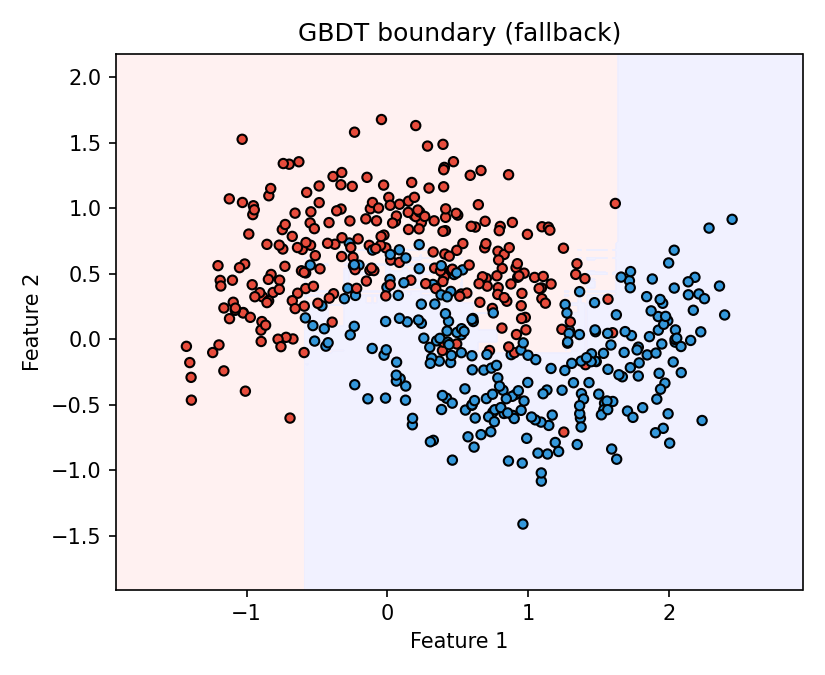
\includegraphics[width=0.9\linewidth]{xgb_decision_boundary_2class.png}
  \caption{XGBoost decision boundary on a 2-class dataset.}
  \label{fig:xgb2}
\end{figure}
\FloatBarrier

\begin{figure}[H]
  \centering
  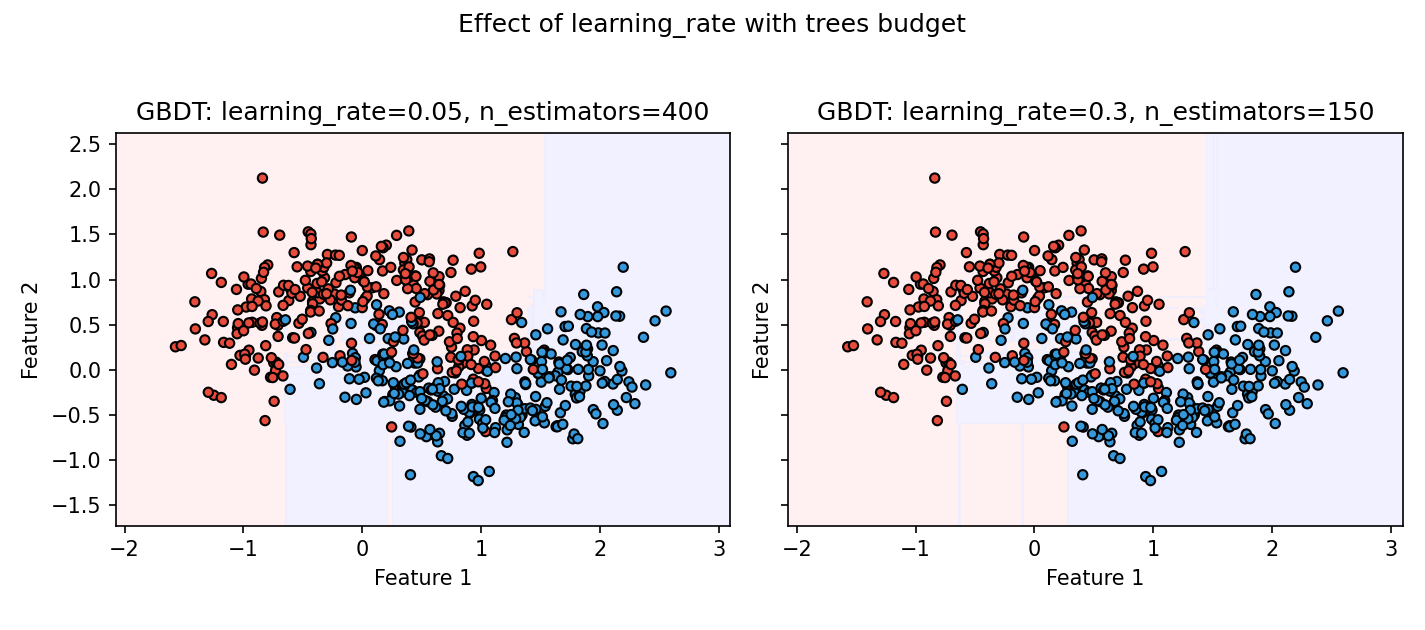
\includegraphics[width=0.95\linewidth]{xgb_learning_rate_compare.png}
  \caption{Learning rate effect with a budget of trees.}
  \label{fig:xgb_lr}
\end{figure}
\FloatBarrier

\begin{figure}[H]
  \centering
  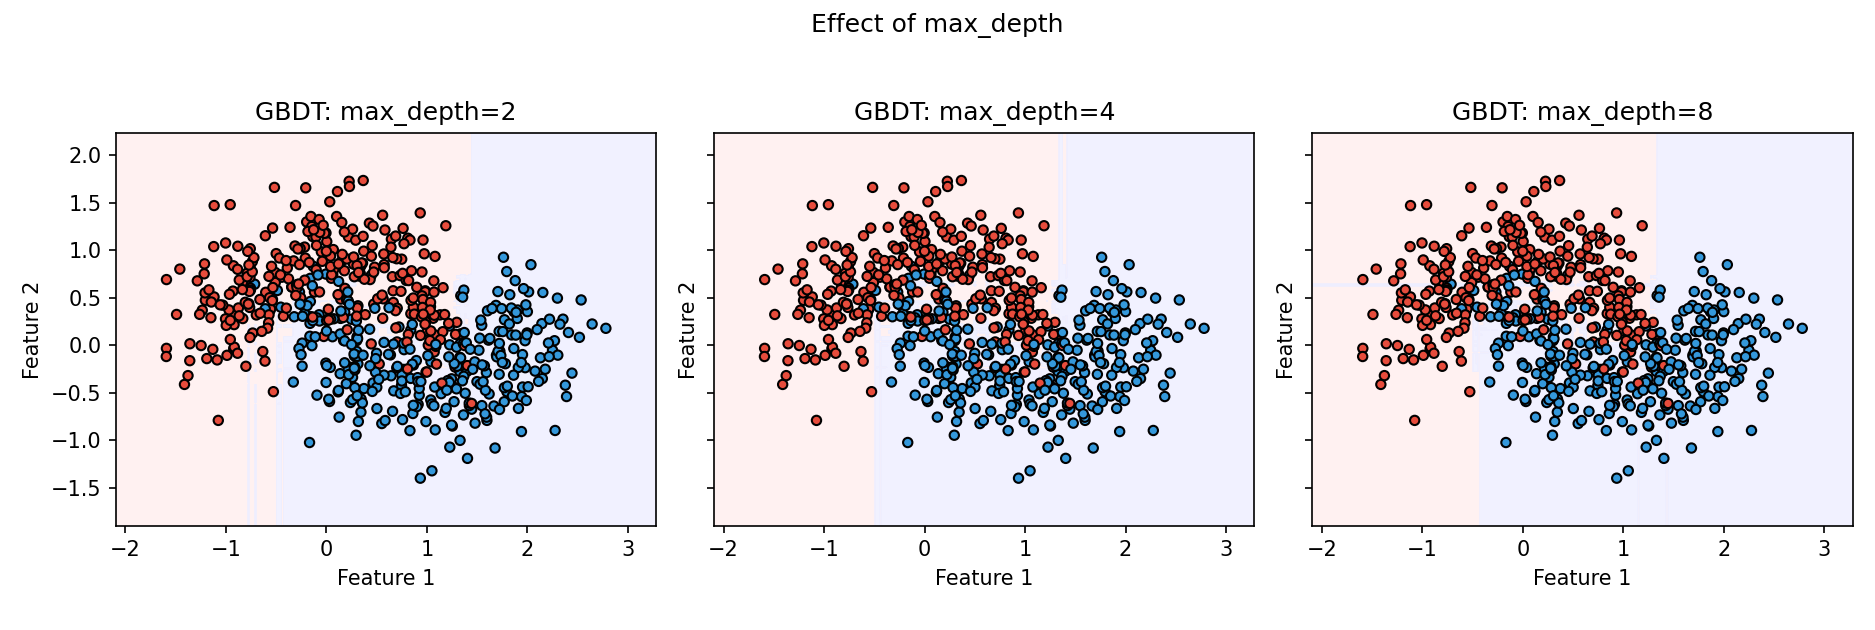
\includegraphics[width=0.95\linewidth]{xgb_max_depth_compare.png}
  \caption{Decision boundaries under different max\_depth.}
  \label{fig:xgb_depth}
\end{figure}
\FloatBarrier

\begin{figure}[H]
  \centering
  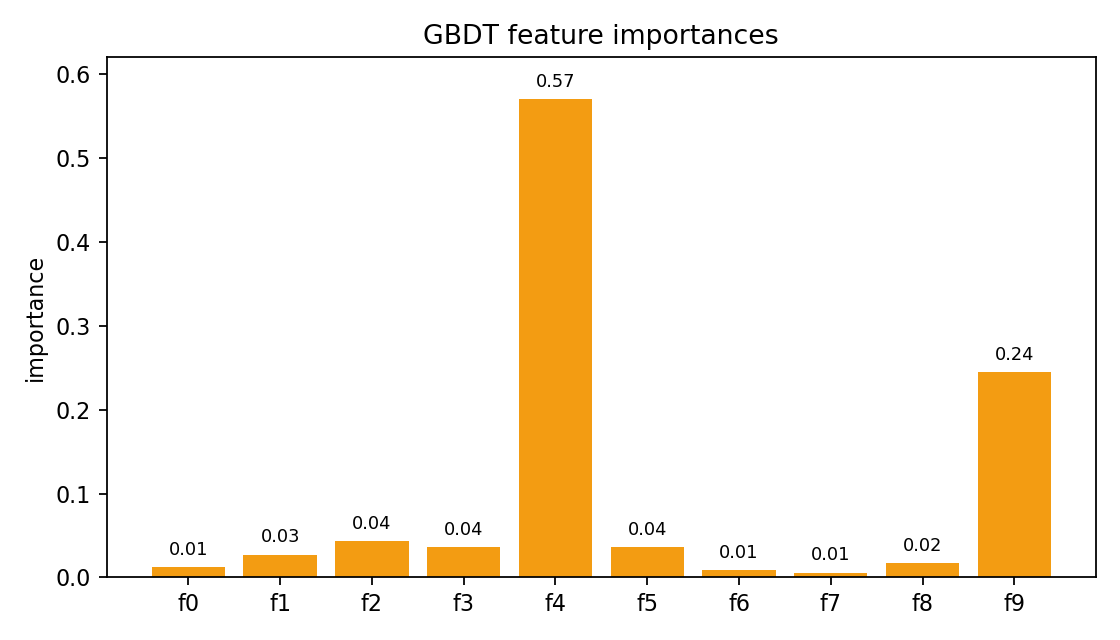
\includegraphics[width=0.85\linewidth]{xgb_feature_importances.png}
  \caption{Feature importances from XGBoost.}
  \label{fig:xgb_fi}
\end{figure}
\FloatBarrier

\begin{figure}[H]
  \centering
  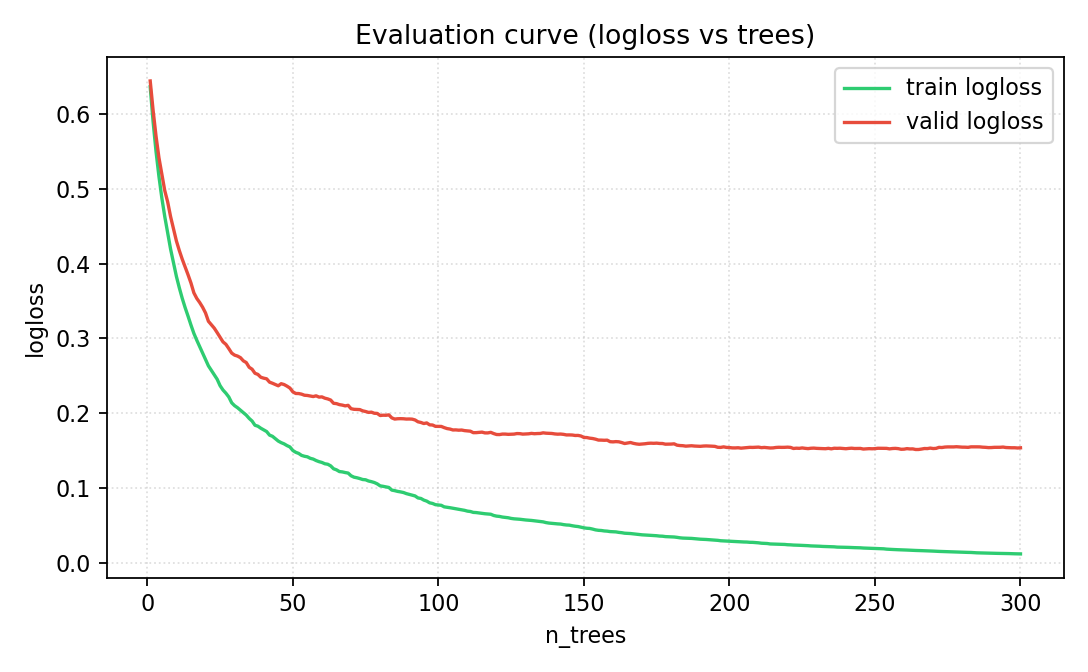
\includegraphics[width=0.85\linewidth]{xgb_eval_logloss_curve.png}
  \caption{Training/validation logloss vs number of trees.}
  \label{fig:xgb_eval}
\end{figure}
\FloatBarrier

\section{Summary}
XGBoost combines efficient tree boosting with strong regularization and advanced split finding. With careful tuning of depth, learning rate, and sampling, it delivers state-of-the-art performance on many tabular tasks.

\end{document}

